\documentclass[11pt,professionalfont,aspectratio=43]{beamer}

% Assets
\usepackage[czech]{babel}				% Jazyk
\usepackage[a-2u]{pdfx}				    % Kopírování z pdfka
\usepackage{tikz}						% Schémata automatů
\usetikzlibrary{shadows, shadows.blur, shapes.geometric, arrows, positioning, overlay-beamer-styles, patterns, shadings, shapes.callouts}
% \usetikzlibrary{arrows}
\usepackage{pgfplots}
% \pgfplotsset{compat=1.15}
% \usepackage{mathrsfs}
\usepackage[export]{adjustbox}

\usepackage[T1]{fontenc}
\usefonttheme[onlymath]{serif}
% \usepackage{newtxmath}
\usepackage{pxfonts}
\usepackage{slantsc}
% \usepackage{varwidth}

\usepackage[linesnumbered,ruled,vlined]{algorithm2e}                % Pseudokód algoritmů
\usepackage[utf8]{inputenc}
% \usepackage{textcomp}
\usepackage{hyperref}
\usepackage{fancybox}

%%% FONTS
% \usefonttheme{serif}
% \usepackage{lmodern}
\usepackage{helvet}

\hypersetup{%
    pdfencoding=auto,
    pdfauthor={\insertauthor},
    pdftitle={\insertsubtitle}
}
\usepackage{float}
\usepackage{csquotes}					% české uvozovky
\usepackage{enumerate}					% enumerate environment
\usepackage{indentfirst}
\usepackage{tcolorbox}                  % Fancy boxíky
\usepackage{mathtools}
\usepackage{pifont}
\usepackage{cancel}
\usepackage{subcaption}
\usepackage{soul}
\usepackage{makecell}                   % Zalomení v buňce tabulky
\usepackage{xcolor}
\usepackage{graphicx}
\usepackage{tabularx}
\usepackage{amsmath}
\usepackage{amsthm}
\usepackage{colortbl}                   % Barvení buněk v tabulce
\usepackage{multicol}                   % Rozdělení obsahu do sloucpů

\usepackage{listings}                   % Úryvky z kódu
\definecolor{maroon}{rgb}{0.5,0,0}
\definecolor{forestgreen}{rgb}{0.13, 0.55, 0.13}

% \lstdefinelanguage{XML}
% {
%   basicstyle=\ttfamily,
%   morestring=[s]{"}{"},
%   morecomment=[s]{?}{?},
%   morecomment=[s]{!--}{--},
%   commentstyle=\color{forestgreen},
%   moredelim=[s][\color{black}]{>}{<},
%   moredelim=[s][\color{red}]{\ }{=},
%   stringstyle=\color{blue},
%   identifierstyle=\color{maroon}
% }
% Colors

\def\maincolR{0} % červená složka (0–255)
\def\maincolG{83} % zelená složka
\def\maincolB{120} % modrá složka
\definecolor{maincolor}{HTML}{8B00B5}

% \pgfmathtruncatemacro{\authorfooterbgR}{1*\maincolR}
% \pgfmathtruncatemacro{\authorfooterbgG}{1*\maincolG}
% \pgfmathtruncatemacro{\authorfooterbgB}{1*\maincolB}
% \definecolor{authorfooterbg}{RGB}{\authorfooterbgR,\authorfooterbgG,\authorfooterbgB}

% \pgfmathtruncatemacro{\titlefooterbgR}{0.722*\maincolR}   
% \pgfmathtruncatemacro{\titlefooterbgG}{0.974*\maincolG}   
% \pgfmathtruncatemacro{\titlefooterbgB}{0.739*\maincolB}
% \definecolor{titlefooterbg}{RGB}{\titlefooterbgR,\titlefooterbgG,\titlefooterbgB}

% Beamer theme
\colorlet{themecolor}{maincolor}
\colorlet{authorfooterbg}{maincolor}
\definecolor{titlefooterbg}{HTML}{9471B0}
\definecolor{titlefooterfg}{HTML}{000000}
\colorlet{titlecolorfg}{maincolor}
\definecolor{titleboxbg}{HTML}{E7E7E7}
\definecolor{datefooterbg}{HTML}{E3E3E3}
\colorlet{titleframeboxcolor}{maincolor}

% Background gradient
\definecolor{gradMiddle}{RGB}{212,248,255}
\definecolor{gradEnd}{RGB}{114,231,255}

% Block theme
\definecolor{blocktitlebg}{HTML}{F0DFA9}
\definecolor{blocktitlefg}{HTML}{957300}
\definecolor{blockbodybg}{HTML}{F5F0DF}

\definecolor{alertblockbodybg}{HTML}{FFE4E4}
\definecolor{alertblocktitlebg}{HTML}{ECA4A4}
\definecolor{alertblocktitlefg}{HTML}{B11313}

\definecolor{exampleblockbodybg}{HTML}{DAF0DA}
\definecolor{exampleblocktitlebg}{HTML}{BBE0BB}
\definecolor{exampleblocktitlefg}{HTML}{257A25}

\definecolor{mathfg}{HTML}{00185E}

\colorlet{bulletbg}{maincolor}
% \definecolor{bulletbg}{HTML}{}

% Beamer theme
\usetheme{Madrid}
\usecolortheme{seahorse}
% \useoutertheme[subsection=false]{miniframes}

\usecolortheme[named=themecolor]{structure}
\setbeamertemplate{frame numbering}[fraction]
\setbeamertemplate{navigation symbols}{}
\setbeamercovered{invisible}

% Header/footer
\setbeamercolor{author in head/foot}{bg=authorfooterbg,fg=white}
\setbeamercolor{title in head/foot}{bg=titlefooterbg,fg=titlefooterfg}
\setbeamercolor{date in head/foot}{bg=datefooterbg,fg=black}
% \setbeamercolor{title}{bg=datefooterbg}
% \setbeamercolor{title}{fg=titlecolorfg}
\setbeamerfont{title}{series=\bfseries}
\setbeamercolor{frametitle}{bg=datefooterbg}
% \setbeamercolor{section in head/foot}{bg=red,fg=cyan}
% \setbeamercolor{subsection in head/foot}{bg=blue,fg=yellow}

% Table of contents
\setbeamercolor{section in toc}{fg=black}
\setbeamercolor{subsection in toc}{fg=red}
\setbeamercolor{section number projected}{fg=black}

% Blocks
\setbeamertemplate{blocks}[rounded][shadow=true]

\setbeamercolor{block title}{bg=blocktitlebg, fg=blocktitlefg}
\setbeamercolor{block body}{parent=normal text,use=block title,bg=blockbodybg}

\setbeamercolor{block body alerted}{bg=alertblockbodybg}
\setbeamercolor{block title alerted}{bg=alertblocktitlebg,fg=alertblocktitlefg}

\setbeamercolor{block body example}{bg=exampleblockbodybg}
\setbeamercolor{block title example}{bg=exampleblocktitlebg,fg=exampleblocktitlefg}

% Math
\setbeamercolor{math text}{fg=mathfg}

% Itemize a enumerate
\setbeamertemplate{itemize items}[circle]
\setbeamertemplate{enumerate items}[circle]
\setbeamercolor{itemize item}{fg=bulletbg,bg=white}
\setbeamercolor{itemize subitem}{fg=bulletbg,bg=white}
\setbeamercolor{itemize subsubitem}{fg=bulletbg,bg=white}

\setbeamertemplate{enumerate items}[circle]
\setbeamercolor{item projected}{bg=bulletbg}

% Titlepage
\defbeamertemplate*{title page}{customized}[1][]
{
    \vbox{}%
    \vfill%
    \begin{centering}
        \begin{tikzpicture}
            \node[thick, rectangle, rounded corners=5mm, drop shadow={shadow xshift=0mm, shadow yshift=2mm, opacity=0.2, blur shadow, shadow blur steps=10}, inner sep=5mm, fill=titleboxbg, fill opacity=1] {%
                {\usebeamerfont{title}\textcolor{titlecolorfg}{\inserttitle}\par}%
            };
        \end{tikzpicture}
        \vskip1em\par%
        \ifx\insertsubtitle\@empty%
        \else%
            {\usebeamerfont{subtitle}\insertsubtitle\par}%
        \fi%
        \vskip1em\par%
        \ifx\insertauthor\@empty%
        \else%
            {\usebeamerfont{author}\insertauthor}\\%
            \texttt{\email}
        \fi
        \vskip0.3em\par%
        % \ifx\insertinstitute\@empty%
        % \else%
        %     {\usebeamerfont{institute}\insertinstitute\par}%
        % \fi%
        \vskip1em\par%
        \ifx\inserttitlegraphic\@empty%
        \else%
            \vskip1em\par%
            \inserttitlegraphic\par%
        \fi%
        \vskip1em\par%
        \ifx\insertdate\@empty%
        \else%
            {\usebeamerfont{date}\insertdate\par}%
        \fi%
    \end{centering}%
    \vfill%
}
% Enumerate
%\setlist[enumerate]{topsep=0pt,itemsep=-1ex,partopsep=1ex,parsep=1ex,label=(\arabic*)}

\MakeOuterQuote{"}

%%% Makra pro definice, věty, tvrzení, příklady, ... (vyžaduje baliček amsthm)

\theoremstyle{plain}
\newtheorem{thm}{Věta}[section]
\newtheorem{lem}[theorem]{Lemma}
\newtheorem{prop}[theorem]{Tvrzení}
\newtheorem{cor}[theorem]{Důsledek}
\newtheorem*{prop*}{Tvrzení}

\theoremstyle{definition}
\newtheorem{define}[theorem]{Definice}
% \newtheorem{example}[theorem]{Příklad}
% \newtheorem{remark}[theorem]{Poznámka}
% \newtheorem{convention}[theorem]{Úmluva}
% \newtheorem{denoting}[theorem]{Značení}

\newenvironment{defblock}[1][]{
  \begin{block}{\ifthenelse{\equal{#1}{}}
  {Definice}
  {Definice (#1)}}
}{\end{block}}
\newenvironment{thmblock}[1][]{
  \begin{block}{\ifthenelse{\equal{#1}{}}
  {Věta}
  {Věta (#1)}}
}{\end{block}}
\newenvironment{corblock}[1][]{
  \begin{block}{\ifthenelse{\equal{#1}{}}
  {Důsledek}
  {Důsledek (#1)}}
}{\end{block}}
\newenvironment{propblock}[1][]{
  \begin{block}{\ifthenelse{\equal{#1}{}}
  {Tvrzení}
  {Tvrzení (#1)}}
}{\end{block}}
\newenvironment{exblock}[1][]{
  \begin{exampleblock}{\ifthenelse{\equal{#1}{}}
  {Příklad}
  {Příklad (#1)}}
}{\end{exampleblock}}


% Colors
\definecolor{lightblue}{HTML}{009AD4}
\definecolor{lightgreen}{HTML}{68FF00}
\definecolor{darkgreen}{HTML}{00B600}
\definecolor{darkblue}{HTML}{0265b3}
\definecolor{darkred}{HTML}{DA0707}
\definecolor{lightred}{HTML}{FF5100}
\definecolor{orange}{HTML}{FFE000}
\definecolor{codeblue}{HTML}{007eed}
\definecolor{codegreen}{rgb}{0,0.6,0}
\definecolor{codegray}{rgb}{0.5,0.5,0.5}
\definecolor{codebeige}{HTML}{D4A000}
\definecolor{codepink}{HTML}{FF0055}
\definecolor{backcolour}{rgb}{0.95,0.95,0.92}

\definecolor{decproblemtitlefg}{HTML}{957300}
\definecolor{decproblembg}{HTML}{F5F0DF}

\definecolor{timportantboxcolor}{HTML}{A97100}
\definecolor{talertboxcolor}{HTML}{B70000}
\definecolor{tnoticeboxcolor}{HTML}{159C00}
\definecolor{tinfoboxcolor}{HTML}{004DFF}

\newcommand{\markred}[1]{\textcolor{lightred}{#1}}
\newcommand{\markdarkred}[1]{\textcolor{darkred}{#1}}
\newcommand{\markgreen}[1]{\textcolor{lightgreen}{#1}}
\newcommand{\markdarkgreen}[1]{\textcolor{darkgreen}{#1}}
\newcommand{\markorange}[1]{\textcolor{orange}{#1}}
\newcommand{\markblue}[1]{\textcolor{lightblue}{#1}}
\newcommand{\markdarkblue}[1]{\textcolor{darkblue}{#1}}

% Math mode settings
% \AtBeginDocument{
%     \setlength{\abovedisplayskip}{3pt}
%     \setlength{\belowdisplayskip}{-4pt}
% }

% Inline images
\newcommand{\inlineimgscale}{1.1}

% X and check mark
\newcommand{\cmark}{\markgreen{\ding{51}}}
\newcommand{\xmark}{\markred{\ding{55}}}

% Math
\newcommand{\R}{\mathbb{R}}
\newcommand{\C}{\mathbb{C}}
\newcommand{\N}{\mathbb{N}}
\newcommand{\Z}{\mathbb{Z}}
\newcommand{\Q}{\mathbb{Q}}

\newcommand{\T}[1]{#1^\top}                     % Tranpozice matice
\newcommand{\compl}[1]{#1^\complement}
\newcommand{\mapping}[3]{#1:#2 \rightarrow #3}
\newcommand{\mapto}[3]{#1:#2 \mapsto #3}
\newcommand{\set}[1]{\left\{#1\right\}}
\newcommand{\powset}{\mathcal{P}}
\newcommand{\code}[1]{\langle#1\rangle}
\DeclareMathOperator*{\argmin}{arg\,min}
\DeclareMathOperator*{\argmax}{arg\,max}

% Statistika a AI
\newcommand{\average}[1]{\overline{#1}}
\DeclareMathOperator{\median}{med}
\DeclareMathOperator{\Var}{var}
\DeclareMathOperator{\Cov}{cov}
\DeclareMathOperator{\MSE}{MSE}
\DeclareMathOperator{\SSE}{SSE}

\DeclareMathOperator{\TP}{TP}
\DeclareMathOperator{\TN}{TN}
\DeclareMathOperator{\FP}{FP}
\DeclareMathOperator{\FN}{FN}
\DeclareMathOperator{\Accuracy}{Acc}
\DeclareMathOperator{\Precision}{Prec}
\DeclareMathOperator{\Recall}{Rec}
\DeclareMathOperator{\Fscore}{F}
\DeclareMathOperator{\Gini}{Gini}

\DeclareMathOperator{\mspan}{span}
\DeclareMathOperator{\mrank}{rank}
\DeclareMathOperator{\tg}{tg}
\DeclareMathOperator{\id}{id}
\DeclareMathOperator{\dom}{dom}
\DeclareMathOperator{\rng}{rng}
\renewcommand{\emptyset}{\varnothing}
\newcommand{\binary}[1]{\ensuremath{\left\langle #1\right\rangle}_B}

% DFS in and out lists
\DeclareMathOperator{\inlist}{in}
\DeclareMathOperator{\outlist}{out}
% \DeclareMathOperator{\lowlist}{low}
\DeclareMathOperator{\key}{key}

% A* macro
\newcommand{\Astar}{$\textcolor{black}{\textup{A}^{*}}$}

% Complexity classes
\DeclareMathOperator{\classP}{P}
\DeclareMathOperator{\classNP}{NP}
\DeclareMathOperator{\classTime}{TIME}
\DeclareMathOperator{\classNTime}{NTIME}
\DeclareMathOperator{\classSpace}{SPACE}
\DeclareMathOperator{\classNSpace}{NSPACE}

\DeclareMathOperator{\SAT}{SAT}
\DeclareMathOperator{\THREESAT}{3-SAT}
\DeclareMathOperator{\UNSAT}{UNSAT}
\DeclareMathOperator{\NZMNA}{NzMna}
\DeclareMathOperator{\KLIKA}{Klika}
\DeclareMathOperator{\ROZVRH}{Rozvrh}
\DeclareMathOperator{\SUDOKU}{Sudoku}
\newcommand{\HALT}{\ensuremath{\textsc{Halt}}}
\newcommand{\FACTOR}{\ensuremath{\textsc{Factor}}}

\DeclareMathOperator{\regex}{RegE}

%%% Barevné boxíky (notice / info / important / alert)
%
% Šířka boxu se nezadává ručně -- box se přizpůsobí šířce svého obsahu.
% Obsah se vysází do prostředí varwidth, takže krátký text zůstane na
% jednom řádku; delší text se zalomí, nejvýše však na šířku \linewidth
% (tj. \textwidth mimo sloupce a minipage). Pokud je titulek širší než
% obsah, řídí šířku boxu titulek.

\newsavebox{\tboxcontentbox}
\newsavebox{\tboxtitlebox}
\newlength{\tboxwidth}
\newlength{\tboxpadding}

% Geometrie boxu (musí odpovídat stylu tautobox níže):
% 2 * (boxrule + boxsep + left)
\setlength{\tboxpadding}{\dimexpr 0.5mm+1mm+4mm\relax}
\setlength{\tboxpadding}{2\tboxpadding}

\tcbset{tautobox/.style={boxrule=0.5mm, boxsep=1mm, left=4mm, right=4mm,
                         fonttitle=\bfseries}}

% Začátek sběru obsahu do boxu
\newcommand{\tboxcollect}{%
  \begin{lrbox}{\tboxcontentbox}%
    \begin{varwidth}{\dimexpr\linewidth-\tboxpadding\relax}%
}

% Ukončení sběru a výpočet výsledné šířky
% #1 = titulek (pro měření; prázdný u variant bez titulku)
\newcommand{\tboxmeasure}[1]{%
    \end{varwidth}%
  \end{lrbox}%
  \sbox{\tboxtitlebox}{\bfseries #1}%
  \setlength{\tboxwidth}{\wd\tboxcontentbox}%
  \ifdim\wd\tboxtitlebox>\tboxwidth
    \setlength{\tboxwidth}{\wd\tboxtitlebox}%
  \fi
  \addtolength{\tboxwidth}{\tboxpadding}%
  \ifdim\tboxwidth>\linewidth
    \setlength{\tboxwidth}{\linewidth}%
  \fi
}

% Vysázení boxu s titulkem: #1 = barva, #2 = titulek
\newcommand{\tboxrenderbox}[2]{%
  \tboxmeasure{#2}%
  \begin{center}%
    \begin{tcolorbox}[tautobox, colback=#1!15, colframe=#1,
                      title={#2}, width=\tboxwidth]
      \usebox{\tboxcontentbox}%
    \end{tcolorbox}%
  \end{center}%
}

% Vysázení boxu bez titulku: #1 = barva
\newcommand{\tboxrenderframe}[1]{%
  \tboxmeasure{}%
  \begin{center}%
    \begin{tcolorbox}[tautobox, colback=#1!15, colframe=#1,
                      width=\tboxwidth]
      \usebox{\tboxcontentbox}%
    \end{tcolorbox}%
  \end{center}%
}

% Poznámky (notice)
\newenvironment{tnoticebox}[1]{%
  \def\tboxtitletext{#1}\tboxcollect
}{%
  \tboxrenderbox{tnoticeboxcolor}{\tboxtitletext}%
}

\newenvironment{tnoticeframe}{%
  \tboxcollect
}{%
  \tboxrenderframe{tnoticeboxcolor}%
}

% Informační bloky (info)
\newenvironment{tinfobox}[1]{%
  \def\tboxtitletext{#1}\tboxcollect
}{%
  \tboxrenderbox{tinfoboxcolor}{\tboxtitletext}%
}

\newenvironment{tinfoframe}{%
  \tboxcollect
}{%
  \tboxrenderframe{tinfoboxcolor}%
}

% Důležité bloky (important)
\newenvironment{timportantbox}[1]{%
  \def\tboxtitletext{#1}\tboxcollect
}{%
  \tboxrenderbox{timportantboxcolor}{\tboxtitletext}%
}

\newenvironment{timportantframe}{%
  \tboxcollect
}{%
  \tboxrenderframe{timportantboxcolor}%
}

% Varovné bloky (alert)
\newenvironment{talertbox}[1]{%
  \def\tboxtitletext{#1}\tboxcollect
}{%
  \tboxrenderbox{talertboxcolor}{\tboxtitletext}%
}

\newenvironment{talertframe}{%
  \tboxcollect
}{%
  \tboxrenderframe{talertboxcolor}%
}

% Decision problem
\newcommand{\decproblem}[3]{
    \begin{center}
        \begin{minipage}{.9\textwidth}
            \begin{table}[!htbp]
                \centering
                \bgroup
                \def\arraystretch{1.8}
                \begin{tabularx}{\textwidth}{|rX|}
                \hline
                \rowcolor{decproblembg} \multicolumn{2}{|c|}{\textcolor{decproblemtitlefg}{\textsc{#1}}} \\ \hline
                \markdarkred{\textbf{Vstup:}} & #2                \\ \hline
                \rowcolor{decproblembg} \markdarkred{\textbf{Otázka:}} & #3               \\ \hline
                \end{tabularx}
                \egroup
            \end{table}
        \end{minipage}
    \end{center}
}
\newcommand{\bigO}{\mathcal{O}}

% TODO
\newcommand{\todo}[1]{\textcolor{red}{(\noindent TODO: #1.)}}


\newcommand{\hlcode}[1]{\colorbox{red}{#1}}

% Algorithms
\numberwithin{algocf}{section}
\renewcommand{\algorithmcfname}{Algoritmus}
\SetKwInput{KwIn}{Vstup}
\SetKwInput{KwOut}{Výstup}
\SetKwProg{Function}{Funkce}{}{end}
\setlength{\algomargin}{25pt}
\renewcommand{\thealgocf}{}     % Vypnutí číslování algoritmů

% Definice stylů pro uzly
\tikzstyle{startstop} = [rectangle, rounded corners, minimum width=1.5cm, minimum height=0.5cm,text centered, draw=black, fill=red!30]
\tikzstyle{process}   = [rectangle, minimum width=1.5cm, minimum height=0.5cm, text centered, draw=black, fill=orange!30]
\tikzstyle{decision}  = [diamond, aspect=2, text centered, draw=black, fill=green!30]
\tikzstyle{arrow}     = [thick,->,>=stealth]

\tikzstyle{vertex}    = [thick, draw, circle, minimum size=4mm, inner sep=1pt, outer sep=1pt, align=center]
\tikzstyle{vertexplain}    = [minimum size=4mm, inner sep=1pt, outer sep=1pt, align=center]
\tikzstyle{verteximg}    = [draw, circle, minimum size=4mm, inner sep=0pt, outer sep=1pt, align=center, clip]
\tikzstyle{verteximgplain}    = [minimum size=4mm, inner sep=0pt, outer sep=1pt, align=center]
\tikzstyle{task}    = [draw, rounded corners=2pt, minimum width=14mm, minimum height=8mm, inner sep=2pt, align=center]

\tikzstyle{edge}    = [thick,>=stealth]
\tikzstyle{diredge}    = [thick, ->, >=stealth]

%% Automaty
\tikzstyle{state}=[%
    draw,
    circle,
    thick,
    minimum size=10mm,
    inner sep=0pt,
    outer sep=0pt
]

\tikzstyle{acceptstate}=[%
    state,
    double,
    double distance=1pt
]

\tikzstyle{transition}=[%
    ->,
    >=stealth,
    thick
]

\newcommand<>{\state}[4][]{%
    \node#5[state,#1] (#2) at #3 {#4};
}

\newcommand<>{\acceptingstate}[4][]{%
    \node#5[acceptstate,#1] (#2) at #3 {#4};
}

\newcommand<>{\transitionarrow}[5][]{%
    \path#6 (#2) edge[transition,#1] node[#3] {#4} (#5);
}

\newcommand<>{\initialstate}[6][]{%
    \node#7[state,#1] (#2) at #3 {#4};
    \draw#7[transition] #5 -- (#2.#6);
}

%%%%%

% Frames
\newcommand{\tableofcontentsframe}{
    \begin{frame}{Obsah}
        \tableofcontents
    \end{frame}
}

% \definecolor{boxcolor}{HTML}{00820a}
\newcommand{\titleframe}[1]{%
  \begin{frame}[plain]
    \begin{tikzpicture}[remember picture, overlay]
      \node at (current page.center)
        [draw=titleframeboxcolor, line width=1pt,
         inner xsep=10mm, inner ysep=4mm, rounded corners=2mm,
         text width=0.8\textwidth, align=center,
         execute at begin node=\setlength{\baselineskip}{2.2em}]
        {\Huge\markred{#1}\normalfont};
    \end{tikzpicture}
  \end{frame}
  \addtocounter{framenumber}{-1}%
}

\newenvironment{titleframeenv}[1]{
    \begin{frame}[plain]
        \begin{tcolorbox}[colback=white,boxrule=1pt]
            \begin{center}
                \Huge\markred{#1}\normalfont
            \end{center}
        \end{tcolorbox}
}{\addtocounter{framenumber}{-1}\end{frame}}

\newcommand{\icon}[1]{
  \includegraphics[height=\fontcharht\font`\B]{#1}
}

% Obrázek, který se vždy vejde na snímek. Adjustbox jej v případě potřeby
% zmenší tak, aby nepřesáhl šířku textu ani zadanou část výšky snímku; díky
% tomu sedí sazba ve všech používaných poměrech stran (4:3, 16:9 i 16:10).
% Volitelným argumentem je maximální výška (výchozí 0.68\textheight), povinným
% cesta k souboru s obrázkem (TikZ zdroj vkládaný přes \input).
\newcommand{\obrazek}[2][0.68\textheight]{%
    \begin{figure}
        \centering
        \begin{adjustbox}{max width=\linewidth, max totalheight=#1, center}
            \input{#2}
        \end{adjustbox}
    \end{figure}%
}

% Totéž pro rastrové či vektorové obrázky vkládané přes \includegraphics.
\newcommand{\obrazekgrf}[2][0.68\textheight]{%
    \begin{figure}
        \centering
        \includegraphics[width=\linewidth, max totalheight=#1, center]{#2}
    \end{figure}%
}

% Závěrečný snímek se seznamem zdrojů. Prvním (volitelným) argumentem je název
% sekce i snímku, druhým čárkou oddělený seznam klíčů z ../assets/literatura.bib.
% Citace se sázejí podle ČSN ISO 690, v pořadí, v jakém jsou klíče uvedeny.
\newcommand{\zdrojeframe}[2][Zdroje]{%
    \section{#1}
    \nocite{#2}%
    \begin{frame}[allowframebreaks]{#1}
        \printbibliography[heading=none]
    \end{frame}
}
\input{../assets/listing.tex}

\def\presentationtitle{Opakování z~teorie grafů}

\begin{document}

    \title[\presentationtitle]{\textsc{Teoretická informatika}}
\subtitle{\presentationtitle}
\author{David Weber}
\def\email{weber3@spsejecna.cz}
\institute{SPŠE Ječná}
\date{%
    Rok 
    \pgfmathsetmacro{\firstyear}{ifthenelse(\month<9, \year-1, \year)}%
    \pgfmathsetmacro{\secondyear}{ifthenelse(\month<9, \year, \year+1)}%
    \pgfmathtruncatemacro{\secondyearlasttwo}{mod(\secondyear,100)}%
    \pgfmathprintnumber[fixed,precision=0,zerofill,1000 sep={}]{\firstyear}/%
    \pgfmathprintnumber[fixed,precision=0,zerofill,1000 sep={}]{\secondyearlasttwo}%
}
\titlegraphic{\includegraphics[width=0.25\textwidth]{../images/SPSE-Jecna_Logo.pdf}}

\begin{frame}[plain]
    \titlepage
\end{frame}

    \section{Teorie grafů}

    \begin{titleframeenv}{Teorie grafů}
        \begin{figure}
            \centering
            \begin{tikzpicture}[scale=1.5]

% vnější vrcholy
\node[vertex, fill=red!35]         (v1) at (90:2)    {};
\node[vertex, fill=orange!40]      (v2) at (18:2)    {};
\node[vertex, fill=yellow!50]      (v3) at (-54:2)   {};
\node[vertex, fill=green!35]       (v4) at (-126:2)  {};
\node[vertex, fill=cyan!35]        (v5) at (162:2)   {};

% vnitřní vrcholy
\node[vertex, fill=blue!35]        (u1) at (90:0.9)    {};
\node[vertex, fill=violet!35]      (u2) at (18:0.9)    {};
\node[vertex, fill=magenta!35]     (u3) at (-54:0.9)   {};
\node[vertex, fill=pink!45]        (u4) at (-126:0.9)  {};
\node[vertex, fill=lime!45]        (u5) at (162:0.9)   {};

% vnější pětiúhelník
\draw[edge] (v1) -- (v2);
\draw[edge] (v2) -- (v3);
\draw[edge] (v3) -- (v4);
\draw[edge] (v4) -- (v5);
\draw[edge] (v5) -- (v1);

% spojky mezi vnějším a vnitřním cyklem
\draw[edge] (v1) -- (u1);
\draw[edge] (v2) -- (u2);
\draw[edge] (v3) -- (u3);
\draw[edge] (v4) -- (u4);
\draw[edge] (v5) -- (u5);

% vnitřní hvězda
\draw[edge] (u1) -- (u3);
\draw[edge] (u3) -- (u5);
\draw[edge] (u5) -- (u2);
\draw[edge] (u2) -- (u4);
\draw[edge] (u4) -- (u1);

\end{tikzpicture}
        \end{figure}
    \end{titleframeenv}

    \subsection{Kde se s~grafy setkáváme}

    \begin{frame}{Kde se s~grafy setkáváme}
        Mapa města a~cesty
        \begin{figure}
            \centering
            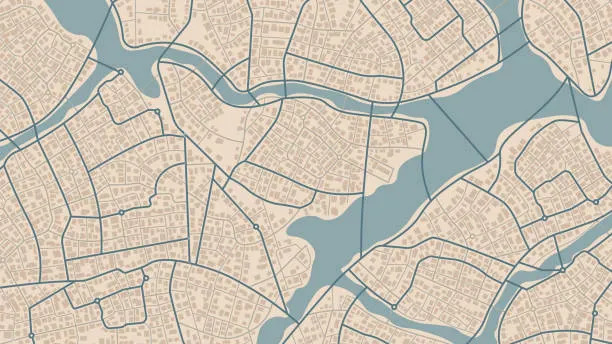
\includegraphics[width=\textwidth]{images/city-map.jpg}
        \end{figure}
    \end{frame}

    \begin{frame}{Kde se s~grafy setkáváme}
        Schéma počítačové sítě
        \begin{figure}
            \centering
            \begin{tikzpicture}[scale=1]

\node[vertexplain] (R)   at (0,-0.5)   {
\includegraphics[width=.1\textwidth]{images/router.png}};
\node[vertexplain] (S1)  at (-2,1) {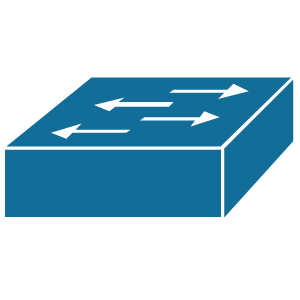
\includegraphics[width=.1\textwidth]{images/workgroup-switch.png}};
\node[vertexplain] (S2)  at (2,1)  {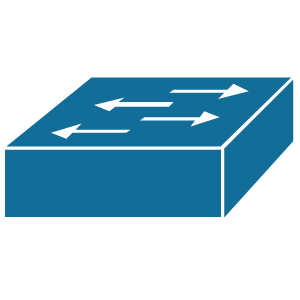
\includegraphics[width=.1\textwidth]{images/workgroup-switch.png}};
\node[vertexplain] (PC1) at (-3.5,3) {
\includegraphics[width=.1\textwidth]{images/vecteezy_3d-monitor-illustration_28537446.png}};
\node[vertexplain] (PC2) at (-1,3)   {
\includegraphics[width=.1\textwidth]{images/vecteezy_3d-monitor-illustration_28537446.png}};
\node[vertexplain] (PC3) at (1,3)    {
\includegraphics[width=.1\textwidth]{images/vecteezy_3d-monitor-illustration_28537446.png}};
\node[vertexplain] (PC4) at (3.5,3)  {
\includegraphics[width=.1\textwidth]{images/vecteezy_3d-monitor-illustration_28537446.png}};
\node[vertexplain] (T)   at (0,-3)   {
\includegraphics[width=.2\textwidth]{images/cloud.png}};

\draw[edge] (R) -- (S1);
\draw[edge] (R) -- (S2);
\draw[edge] (R) -- (T);
\draw[edge] (S1) -- (PC1);
\draw[edge] (S1) -- (PC2);
\draw[edge] (S2) -- (PC3);
\draw[edge] (S2) -- (PC4);

\end{tikzpicture}

        \end{figure}
    \end{frame}

    \subsection{Definice grafu}

    \begin{frame}{Grafy formálně}
        \visible<2->{
            \begin{defblock}[Neorientovaný graf]
                \markdarkred{Neorientovaným grafem} $G$ nazveme uspořádanou dvojici $(V,E)$, kde
                \begin{itemize}
                    \item $V$ je množina \textbf{vrcholů} a
                    \item $E\subseteq\set{\set{u,v}: u,v\in V}$ je množina \textbf{hran}.
                \end{itemize}
            \end{defblock}
        }

        \visible<3->{
            Pokud chceme, aby hrany byly \markdarkred{orientované}, stačí v~definici upravit množinu $E$ takto:
            \[E\subseteq\set{(u,v): u,v\in V}.\]
        }
    \end{frame}

    \begin{frame}{Příklad}{Neorientovaný graf}
        \begin{figure}
            \centering
            \begin{tikzpicture}[scale=1]

\node[vertex,fill=red] (VI1)   at (-1,-1) {};
\node[vertex,fill=red] (VI2)   at (1,-1) {};
\node[vertex,fill=red] (VI3)   at (1,1) {};
\node[vertex,fill=red] (VI4)   at (-1,1) {};

\node[vertex,fill=red] (VO1)   at (-2,-2) {};
\node[vertex,fill=red] (VO2)   at (2,-2) {};
\node[vertex,fill=red] (VO3)   at (2,2) {};
\node[vertex,fill=red] (VO4)   at (-2,2) {};

\draw[edge] (VI1) -- (VI2);
\draw[edge] (VI2) -- (VI3);
\draw[edge] (VI3) -- (VI4);
\draw[edge] (VI4) -- (VI1);
\draw[edge] (VI4) -- (VI2);
\draw[edge] (VI3) -- (VI1);

\draw[edge] (VO4) -- (VI4);
\draw[edge] (VO3) -- (VI3);
\draw[edge] (VO2) -- (VI2);
\draw[edge] (VO1) -- (VI1);


\draw[edge] (VO1) -- (VO2);
\draw[edge] (VO2) -- (VO3);
\draw[edge] (VO3) -- (VO4);
\draw[edge] (VO4) -- (VO1);

\end{tikzpicture}

        \end{figure}
    \end{frame}

    \begin{frame}{Příklad}{{Orientovaný graf}}
        \begin{figure}
            \centering
            \begin{tikzpicture}[scale=1]

\node[vertex,fill=orange] (VI1)   at (-1,-1) {};
\node[vertex,fill=orange] (VI2)   at (1,-1) {};
\node[vertex,fill=orange] (VI3)   at (1,1) {};
\node[vertex,fill=orange] (VI4)   at (-1,1) {};

\node[vertex,fill=orange] (VO1)   at (-2,-2) {};
\node[vertex,fill=orange] (VO2)   at (2,-2) {};
\node[vertex,fill=orange] (VO3)   at (2,2) {};
\node[vertex,fill=orange] (VO4)   at (-2,2) {};

\draw[diredge] (VI1) -- (VI2);
\draw[diredge] (VI2) -- (VI3);
\draw[diredge] (VI3) -- (VI4);
\draw[diredge] (VI4) -- (VI1);
\draw[diredge] (VI4) -- (VI2);
\draw[diredge] (VI3) -- (VI1);

\draw[diredge] (VO4) -- (VI4);
\draw[diredge] (VO3) -- (VI3);
\draw[diredge] (VO2) -- (VI2);
\draw[diredge] (VO1) -- (VI1);


\draw[diredge] (VO1) -- (VO2);
\draw[diredge] (VO2) -- (VO3);
\draw[diredge] (VO3) -- (VO4);
\draw[diredge] (VO4) -- (VO1);

\end{tikzpicture}

        \end{figure}
    \end{frame}

    \begin{frame}{Incidence}
        \visible<2->{\begin{defblock}[Incidence]
            Nechť $G=(V,E)$ je graf, $u\in V$ a~$e\in E$. Pak říkáme, že $e$ je incidentní s~vrcholem $u$, když je $u$ jedním z~koncových vrcholů hrany $e$.
        \end{defblock}}
        \visible<3->{\begin{figure}
            \centering
            \begin{tikzpicture}[scale=1]

    \node[vertex,fill=green] (V)   at (0,0) {$v$};
    \node[vertexplain] (VP1)   at (2,1) {};
    \node[vertexplain] (VP2)   at (2,0) {};
    \node[vertexplain] (VP3)   at (2,-1) {};
    \node[vertexplain] (VP4)   at (-2,1) {};
    \node[vertexplain] (VP5)   at (-2,0) {};
    \node[vertexplain] (VP6)   at (-2,-1) {};
    
    \node[vertexplain] (Vdots1)   at (-2.5,0) {$\dots$};
    \node[vertexplain] (Vdots2)   at (2.5,0) {$\dots$};
    \node[vertexplain] (Vdots1)   at (-2.5,-1) {$\dots$};
    \node[vertexplain] (Vdots2)   at (2.5,-1) {$\dots$};
    \node[vertexplain] (Vdots1)   at (-2.5,1) {$\dots$};
    \node[vertexplain] (Vdots2)   at (2.5,1) {$\dots$};

    \draw[edge] (V) -- (VP1);
    \draw[edge] (V) -- (VP2);
    \draw[edge] (V) -- (VP3);
    \draw[edge] (V) -- (VP4);
    \draw[edge] (V) -- (VP5);
    \draw[edge] (V) -- (VP6);

\end{tikzpicture}

        \end{figure}}
    \end{frame}

    \subsection{Vzdálenosti}

    \begin{frame}{Vzdálenosti vrcholů}
        \visible<2->{\begin{defblock}[Dosažitelný vrchol]
            Nechť \(G=(V,E)\) je graf a \(u,v\in V\). Řekneme, že $v$ je \markdarkred{dosažitelný} z vrcholu $u$, pokud \textbf{existuje cesta} z vrcholu $u$ do vrcholu $v$.
        \end{defblock}}
        \visible<3->{\begin{defblock}[Vzdálenost vrcholů]
            Nechť \(G=(V,E)\) je graf a \(u,v\in V\). \markdarkred{Vzdálenost vrcholů} \(u\) a \(v\), značená \(d(u,v)\), je \textbf{délka nejkratší cesty} z vrcholu \(u\) do vrcholu \(v\) měřená počtem jejích hran, existuje-li taková cesta. Pokud cesta z \(u\) do \(v\) neexistuje, definujeme $d(u,v)=\infty$.
        \end{defblock}}
        \visible<4->{Pro neorientované grafy je vzdálenost symetrická, tzn.
        \[d(u,v)=d(v,u).\]}
        \visible<5->{\begin{talertframe}
            \begin{center}
                Pro \textbf{orientované grafy} to samé ale nemusí platit!
            \end{center}
        \end{talertframe}}
    \end{frame}

    \begin{frame}{Asymetričnost vzdálenosti vrcholů}{Příklad}
        \begin{figure}
            \centering
            \begin{tikzpicture}[scale=1.2]

\node[vertex] (u) at (0,0) {$u$};
\node[vertex] (a) at (2,1.5) {$w$};
\node[vertex] (v) at (4,0) {$v$};

\draw[diredge] (u) -- (a);
\draw[diredge] (a) -- (v);
\draw[diredge] (v) to[bend right=25] (u);

\end{tikzpicture}
        \end{figure}
        \visible<2>{\[d(u,v)=2,\qquad d(v,u)=1.\]}
    \end{frame}

    \section{Reprezentace grafů}

    \titleframe{Reprezentace grafů}

    \subsection{Matice}

    \begin{frame}{Matice}
        \visible<2->{
            \markdarkred{Maticí} $\mathbf{A}$ typu $n\times m$ rozumíme blokové schéma
            \[
            \mathbf{A}=
            \left(
            \begin{matrix}
                a_{11} & a_{12} & \ldots & a_{1m} \\
                a_{21} & a_{22} & \ldots & a_{2m} \\
                \vdots & \vdots & \ddots & \vdots \\
                a_{n1} & a_{n2} & \ldots & a_{nm}
            \end{matrix}
            \right)
            \]
        }
        \visible<3->{Prvek matice $\mathbf{A}$ na pozici $(i,j)$ značíme $\mathbf{A}_{ij}$.}

        \visible<4->{\begin{exblock}
        Matice
        \[\mathbf{A}=\left(\begin{matrix}
            1 & 2 & 3 \\
            4 & 5 & 6 \\
            7 & 8 & 9
        \end{matrix}\right),\; \mathbf{B}=\left(\begin{matrix}
            1 & -1 & 2 & -2 \\
            3 & -3 & -4 & 4
        \end{matrix}\right)\]
        jsou po řadě typů $3\times 3$ a~$2\times 4$.
        \end{exblock}}
    \end{frame}

    \begin{frame}{Reprezentace grafu}
        \visible<2->{Máme libovolný graf $G=(V,E)$. Rádi bych co nejrychleji zjistili pro zadaný vrchol $u\in V$, do jakých vrcholů se z~něj můžeme dostat.}
        \visible<3->{\begin{talertframe}
            \begin{center}
                Přímá definice není moc praktická.
            \end{center}
        \end{talertframe}}
        \visible<4->{\begin{figure}
                \centering
                \begin{tikzpicture}[scale=1]

\node[vertex,fill=white] (V1)   at (-1,-1) {$v_1$};
\node[vertex,fill=white] (V2)   at (0,0) {$v_2$};
\node[vertex,fill=white] (V3)   at (0,1) {$v_3$};
\node[vertex,fill=white] (V4)   at (2,1) {$v_4$};
\node[vertex,fill=white] (V5)   at (3,0) {$v_5$};
\node[vertex,fill=white] (V6)   at (2,-1) {$v_6$};

\draw[edge] (V1) -- (V2);
\draw[edge] (V2) -- (V3);
\draw[edge] (V3) -- (V4);
\draw[edge] (V4) -- (V5);
\draw[edge] (V5) -- (V6);
\draw[edge] (V4) -- (V2);
\draw[edge] (V2) -- (V6);

\end{tikzpicture}
            \end{figure}}
        \visible<5->{Grafy můžeme reprezentovat třemi způsoby:}
        \visible<6->{\begin{itemize}
            \visible<6->{\item \markdarkred{maticí sousednosti},}
            \visible<7->{\item \markdarkred{maticí incidence} a}
            \visible<8->{\item \markdarkred{seznamy sousedních vrcholů}.}
        \end{itemize}}
    \end{frame}

    \subsection{Matice sousednosti}

    \begin{frame}{Matice sousednosti}
        \begin{itemize}
            \visible<2->{\item Mějme \textbf{orientovaný} nebo \textbf{neorientovaný} graf $G=(V,E)$, přičemž
            \[V=\set{v_1,v_2,\dots,v_n}.\]}
            \visible<3->{\item Definujeme prvky matice $\mathbf{A}$ typu $n\times n$ pro každé $i,j\in\set{1,\dots,n}$ předpisem
            \[\mathbf{A}_{ij}=\begin{cases}
                1 & \text{vede-li z~vrcholu $v_i$ hrana do vrcholu $v_j$},\\
                0 & \text{jinak}.
            \end{cases}\]}
            \visible<4->{Matice $\mathbf{A}$ je tzv. \markdarkred{maticí sousednosti} grafu $G$.}
        \end{itemize}
    \end{frame}

    \begin{frame}{Matice sousednosti}{Příklad \textrm{I}}
        \visible<2->{\begin{minipage}{0.45\textwidth}
            Graf $G$
            \begin{figure}
                \centering
                \begin{tikzpicture}[scale=1]

\node[vertex,fill=white] (V1)   at (-1,-1) {$v_1$};
\node[vertex,fill=white] (V2)   at (0,0) {$v_2$};
\node[vertex,fill=white] (V3)   at (0,1) {$v_3$};
\node[vertex,fill=white] (V4)   at (2,1) {$v_4$};
\node[vertex,fill=white] (V5)   at (3,0) {$v_5$};
\node[vertex,fill=white] (V6)   at (2,-1) {$v_6$};

\draw[edge] (V1) -- (V2);
\draw[edge] (V2) -- (V3);
\draw[edge] (V3) -- (V4);
\draw[edge] (V4) -- (V5);
\draw[edge] (V5) -- (V6);
\draw[edge] (V4) -- (V2);
\draw[edge] (V2) -- (V6);

\end{tikzpicture}
            \end{figure}
        \end{minipage}}
        \visible<3->{\begin{minipage}{0.45\textwidth}
            \begin{table}
                \centering
                \begin{tabular}{c|cccccc}
                    $\mathbf{A}_G$ & $v_1$ & $v_2$ & $v_3$ & $v_4$ & $v_5$ & $v_6$ \\ \hline
                    $v_1$ & \visible<4->{$0$ & $1$ & $0$ & $0$ & $0$ & $0$ \\}
                    $v_2$ & \visible<5->{$1$ & $0$ & $1$ & $1$ & $0$ & $1$ \\}
                    $v_3$ & \visible<6->{$0$ & $1$ & $0$ & $1$ & $0$ & $0$ \\}
                    $v_4$ & \visible<7->{$0$ & $1$ & $1$ & $0$ & $1$ & $0$ \\}
                    $v_5$ & \visible<8->{$0$ & $0$ & $0$ & $1$ & $0$ & $1$ \\}
                    $v_6$ & \visible<9->{$0$ & $1$ & $0$ & $0$ & $1$ & $0$}
                \end{tabular}
            \end{table}
        \end{minipage}}
        \visible<10->{Výsledná matice sousednosti grafu $G$:
        \[\mathbf{A}_G=\left(\begin{matrix}
            0 & 1 & 0 & 0 & 0 & 0 \\
            1 & 0 & 1 & 1 & 0 & 1 \\
            0 & 1 & 0 & 1 & 0 & 0 \\
            0 & 1 & 1 & 0 & 1 & 0 \\
            0 & 0 & 0 & 1 & 0 & 1 \\
            0 & 1 & 0 & 0 & 1 & 0
        \end{matrix}\right)\]}
    \end{frame}

    \begin{frame}{Matice sousednosti}{Příklad \textrm{II}}
        \visible<2>{Graf $H$ (prasátko)
        \begin{figure}
            \centering
            \input{images/graf-prasatko.tex}
        \end{figure}}
    \end{frame}

    \begin{frame}{Matice sousednosti}{Příklad \textrm{II}}
        \begin{table}
            \centering
            \begin{tabular}{c|cccccccccc}
                $\mathbf{A}_H$ & $v_0$ & $v_1$ & $v_2$ & $v_3$ & $v_4$ & $v_5$ & $v_6$ & $v_7$ & $v_8$ & $v_9$ \\ \hline
                $v_0$ & $0$ & $1$ & $0$ & $1$ & $0$ & $0$ & $0$ & $0$ & $0$ & $1$ \\
                $v_1$ & $0$ & $0$ & $1$ & $1$ & $0$ & $0$ & $0$ & $0$ & $0$ & $0$ \\
                $v_2$ & $0$ & $0$ & $0$ & $0$ & $0$ & $0$ & $0$ & $0$ & $0$ & $0$ \\
                $v_3$ & $0$ & $0$ & $0$ & $0$ & $1$ & $0$ & $0$ & $0$ & $0$ & $0$ \\
                $v_4$ & $0$ & $0$ & $0$ & $0$ & $0$ & $0$ & $0$ & $0$ & $0$ & $0$ \\
                $v_5$ & $0$ & $0$ & $0$ & $1$ & $0$ & $0$ & $0$ & $0$ & $0$ & $0$ \\
                $v_6$ & $1$ & $0$ & $0$ & $1$ & $0$ & $0$ & $0$ & $1$ & $0$ & $0$ \\
                $v_7$ & $0$ & $0$ & $0$ & $0$ & $0$ & $0$ & $0$ & $0$ & $0$ & $0$ \\
                $v_8$ & $0$ & $0$ & $0$ & $0$ & $0$ & $0$ & $1$ & $0$ & $0$ & $0$ \\
                $v_9$ & $0$ & $0$ & $0$ & $0$ & $0$ & $0$ & $1$ & $0$ & $0$ & $0$
            \end{tabular}
        \end{table}
    \end{frame}

    \begin{frame}{Matice sousednosti}{Příklad \textrm{II}}
        Výsledná matice sousednosti grafu $H$:
        \[\mathbf{A}_H=\left(\begin{matrix}
            0 & 1 & 0 & 1 & 0 & 0 & 0 & 0 & 0 & 1 \\
            0 & 0 & 1 & 1 & 0 & 0 & 0 & 0 & 0 & 0 \\
            0 & 0 & 0 & 0 & 0 & 0 & 0 & 0 & 0 & 0 \\
            0 & 0 & 0 & 0 & 1 & 0 & 0 & 0 & 0 & 0 \\
            0 & 0 & 0 & 0 & 0 & 0 & 0 & 0 & 0 & 0 \\
            0 & 0 & 0 & 1 & 0 & 0 & 0 & 0 & 0 & 0 \\
            1 & 0 & 0 & 1 & 0 & 0 & 0 & 1 & 0 & 0 \\
            0 & 0 & 0 & 0 & 0 & 0 & 0 & 0 & 0 & 0 \\
            0 & 0 & 0 & 0 & 0 & 0 & 1 & 0 & 0 & 0 \\
            0 & 0 & 0 & 0 & 0 & 0 & 1 & 0 & 0 & 0
        \end{matrix}\right)\]
    \end{frame}

    \begin{frame}{Poznámka k~matici sousednosti}
        \visible<2->{Všimněme si, že matice sousednosti $A$ \textbf{neorientovaného grafu} je vždy \markdarkred{symetrická}, tzn.~pro každé $i,j$ platí
        \[\mathbf{A}_{ij}=\mathbf{A}_{ji}.\]}
        \visible<3->{\begin{talertframe}
            U~neorientovaného grafu nám tedy stačí vyplnit horní polovinu matice $\implies$ zbytek vznikne "zrcadlením" podle hlavní diagonály.
        \end{talertframe}}
    \end{frame}

    \subsection{Matice incidence}

    \begin{frame}{Matice incidence}
        \visible<2->{\begin{itemize}
            \visible<2->{\item Mějme graf $G=(V,E)$, kde
            \[V=\set{v_1,v_2,\dots,v_n}\quad\text{a}\quad E=\set{e_1,e_2,\dots,e_m}.\]}
            \visible<3->{\item Definujeme prvky matice $\mathbf{I}$ typu $n\times m$ pro každé $i\in\set{1,\dots,n}$ a~$j\in\set{1,\dots,m}$ následovně:}
            \visible<4->{\begin{itemize}
                \visible<4->{\item Je-li graf $G$ \markdarkred{orientovaný}, pak
                \[\mathbf{I}_{ij}=\begin{cases}
                    -1 & \text{vede-li \textbf{z} vrcholu $v_i$ hrana $e_j$}, \\
                    1 & \text{vede-li \textbf{do} vrcholu $v_i$ hrana $e_j$}, \\
                    0 & \text{jinak}.
                \end{cases}\]}
                \visible<5->{\item Je-li graf $G$ \markdarkred{neorientovaný}, pak
                \[\mathbf{I}_{ij}=\begin{cases}
                    1 & \text{je-li hrana $e_i$ incidentní s~vrcholem $v_i$}, \\
                    0 & \text{jinak}.
                \end{cases}\]}
            \end{itemize}}
        \end{itemize}}
        \visible<6->{Matice $\mathbf{I}$ je tzv. \markdarkred{maticí incidence} grafu $G$.}
    \end{frame}

    \begin{frame}{Matice incidence}{Příklad \textrm{I}}
        \visible<2->{\begin{minipage}{0.45\textwidth}
            Graf $G$
            \begin{figure}
                \centering
                \begin{tikzpicture}[scale=1]

\node[vertex,fill=white] (V1)   at (-2,0) {$u_1$};
\node[vertex,fill=white] (V2)   at (0,0) {$u_2$};
\node[vertex,fill=white] (V3)   at (0,2) {$u_3$};

\node[vertex,fill=white] (V4)   at (1,0) {$u_4$};
\node[vertex,fill=white] (V5)   at (3,0) {$u_5$};
\node[vertex,fill=white] (V6)   at (1,2) {$u_6$};

\draw[diredge] (V1) -- node[midway,above] {$e_1$} (V2);
\draw[diredge] (V1) -- node[midway,above] {$e_2$} (V3);
\draw[diredge] (V2) -- node[midway,right] {$e_3$} (V3);

\draw[diredge] (V4) -- node[midway,above] {$e_4$} (V5);
\draw[diredge] (V6) -- node[midway,right] {$e_5$} (V4);
\draw[diredge] (V5) -- node[midway,above] {$e_6$} (V6);

\end{tikzpicture}
            \end{figure}
        \end{minipage}}
        \visible<3->{\begin{minipage}{0.45\textwidth}
            \begin{table}
                \centering
                \begin{tabular}{c|cccccc}
                    $\mathbf{I_G}$ & $e_1$ & $e_2$ & $e_3$ & $e_4$ & $e_5$ & $e_6$ \\ \hline
                    $u_1$ & \visible<4->{$-1$ & $-1$ & $0$ & $0$ & $0$ & $0$ \\}
                    $u_2$ & \visible<5->{$1$ & $0$ & $-1$ & $0$ & $0$ & $0$ \\}
                    $u_3$ & \visible<6->{$0$ & $1$ & $1$ & $0$ & $0$ & $0$ \\}
                    $u_4$ & \visible<7->{$0$ & $0$ & $0$ & $-1$ & $1$ & $0$ \\}
                    $u_5$ & \visible<8->{$0$ & $0$ & $0$ & $1$ & $0$ & $-1$ \\}
                    $u_6$ & \visible<9->{$0$ & $0$ & $0$ & $0$ & $-1$ & $1$}
                \end{tabular}
            \end{table}
        \end{minipage}}
        \visible<10->{Výsledná matice incidence grafu $G$:
        \[\mathbf{I_G}=\left(\begin{matrix}
            -1 & -1 & 0 & 0 & 0 & 0 \\
            1 & 0 & -1 & 0 & 0 & 0 \\
            0 & 1 & 1 & 0 & 0 & 0 \\
            0 & 0 & 0 & -1 & 1 & 0 \\
            0 & 0 & 0 & 1 & 0 & -1 \\
            0 & 0 & 0 & 0 & -1 & 1
        \end{matrix}\right)\]}
    \end{frame}

    \subsection{Seznamy sousedů}

    \begin{frame}{Seznamy sousedů}
        \begin{itemize}
            \visible<2->{\item Patrně nejznámější způsob reprezentace grafu.}
            \visible<2->{\item Pro graf $G=(V,E)$ definujeme \markdarkred{seznam sousedů} vrcholu $v\in V$ jako množinu
            \[S[v]=\set{u\in V: \text{Z vrcholu $v$ vede hrana do $u$}}.\]}
        \end{itemize}
    \end{frame}

    \begin{frame}{Seznamy sousedů}{Příklad \textrm{II}}
        \visible<2->{Prasátkový graf a~seznamy sousedů jeho vrcholů
        \begin{figure}
            \centering
            \input{images/graf-prasatko.tex}
        \end{figure}}
        \begin{minipage}{0.3\textwidth}
            \begin{align*}
                \visible<3->{S[v_0]&=\set{v_1,v_3} \\ }
                \visible<4->{S[v_1]&=\set{v_2,v_3} \\ }
                \visible<5->{S[v_2]&=\emptyset \\ }
                \visible<6->{S[v_3]&=\set{v_4}}
            \end{align*}
        \end{minipage}
        \begin{minipage}{0.3\textwidth}
            \begin{align*}
                \visible<7->{S[v_4]&=\emptyset \\}
                \visible<8->{S[v_5]&=\set{v_3} \\ }
                \visible<9->{S[v_6]&=\set{v_0,v_3,v_7} \\ }
                \visible<10->{S[v_7]&=\emptyset}
            \end{align*}
        \end{minipage}
        \begin{minipage}{0.3\textwidth}
            \begin{align*}
                \visible<11->{S[v_8]&=\set{v_6} \\}
                \visible<12->{S[v_9]&=\set{v_6}}
            \end{align*}
        \end{minipage}
    \end{frame}

    \section{Stupeň vrcholu a~princip sudosti}

    \titleframe{Princip sudosti}

    \subsection{Stupeň vrcholu}

    \begin{frame}{Stupeň vrcholu}
        \begin{defblock}[Stupeň vrcholu]
            Nechť $G=(V,E)$ je neorientovaný graf a~$v\in V$ jeho libovolný vrchol. Pak definujeme \markdarkred{stupeň vrcholu $v$}
            \[\deg{v}=|\set{e\in E: u\in e}|.\]
        \end{defblock}
    \end{frame}

    \begin{frame}{Stupeň vrcholu v orintovaném grafu}
        \begin{defblock}[Stupeň vrcholu]
            Nechť $G=(V,E)$ je orientovaný graf a~$v\in V$ jeho libovolný vrchol. Pak definujeme
            \begin{itemize}
                \item \markdarkred{vstupní stupeň vrcholu $v$}
                \[\deg^{+}{v}=|\set{e\in E: \exists u\in V: e=(u,v)}|\]
                \item \markdarkred{výstupní stupeň vrcholu $v$}
                \[\deg^{-}{v}=|\set{e\in E: \exists u\in V: e=(v,u)}|.\]
                \item \markdarkred{stupeň vrcholu $v$} jako $\deg{v}=\deg^{+}{v}+\deg^{-}{v}$.
            \end{itemize}
        \end{defblock}
    \end{frame}

    \begin{frame}{Stupeň vrcholu}{Příklad}
        \visible<2->{\begin{figure}
            \centering
            \begin{tikzpicture}[scale=1.2]

\node[vertex] (v1) at (0,2) {$v_1$};
\node[vertex] (v2) at (2,3) {$v_2$};
\node[vertex] (v3) at (2,1) {$v_3$};
\node[vertex] (v4) at (4,3) {$v_4$};
\node[vertex] (v5) at (4,1) {$v_5$};

\draw[edge] (v1) -- (v2);
\draw[edge] (v1) -- (v3);
\draw[edge] (v2) -- (v3);
\draw[edge] (v2) -- (v4);
\draw[edge] (v3) -- (v5);
\draw[edge] (v4) -- (v5);

\visible<3>{\node[above left=2mm and -1mm of v1] {\small $\deg{v_1}=2$};
\node[above=2mm of v2]               {\small $\deg{v_2}=3$};
\node[below=2mm of v3]               {\small $\deg{v_3}=3$};
\node[above=2mm of v4]               {\small $\deg{v_4}=2$};
\node[below=2mm of v5]               {\small $\deg{v_5}=2$};}

\end{tikzpicture}

        \end{figure}}
    \end{frame}

    % \begin{frame}{Vstupní a~výstupní stupeň vrcholu}{Příklad}
    %     \visible<2->{\begin{figure}
    %         \centering
    %         \begin{tikzpicture}[scale=1.2]

    %         \node[vertex] (v1) at (0,2) {$v_1$};
    %         \node[vertex] (v2) at (2,3) {$v_2$};
    %         \node[vertex] (v3) at (2,1) {$v_3$};
    %         \node[vertex] (v4) at (4,3) {$v_4$};
    %         \node[vertex] (v5) at (4,1) {$v_5$};

    %         \draw[diredge] (v1) -- (v2);
    %         \draw[diredge] (v1) -- (v3);
    %         \draw[diredge] (v2) -- (v4);
    %         \draw[diredge] (v3) -- (v2);
    %         \draw[diredge] (v3) -- (v5);
    %         \draw[diredge] (v4) -- (v5);
    %         \draw[diredge] (v5) to[bend left=18] (v2);

    %         \visible<3>{\node[above=2mm of v1] {\tiny $\deg^+(v_1)=2,\ \deg^-(v_1)=0$};
    %         \node[above=4mm of v2]               {\tiny $\deg^+(v_2)=1,\ \deg^-(v_2)=3$};
    %         \node[below=4mm of v3]               {\tiny $\deg^+(v_3)=2,\ \deg^-(v_3)=1$};
    %         \node[above=1mm of v4]               {\tiny $\deg^+(v_4)=1,\ \deg^-(v_4)=1$};
    %         \node[below=1mm of v5]               {\tiny $\deg^+(v_5)=1,\ \deg^-(v_5)=2$};}

    %         \end{tikzpicture}
    %     \end{figure}}
    % \end{frame}

    \begin{frame}{Poznámky k~definici \textrm{I}}
        \begin{itemize}
            \visible<2->{\item Definice říká, že stupeň vrcholu $v$ je jednoduše počet hran incidentních s~$v$.}
            \visible<3->{\item Vstupní a~výstupní stupeň vrcholu $v$ je počet všech hran vycházejících, resp. přicházejících do vrcholu $v$.}
        \end{itemize}
    \end{frame}

    \begin{frame}{Poznámky k~definici \textrm{II}}
        \visible<2->{\begin{tinfobox}{Pozorování}
            Je-li $\mathbf{A}$ matice sousednosti, resp. $\mathbf{I}$ matice incidence, \textbf{neorientovaného} grafu $G$, pak pro libovolný jeho vrchol $v_i$ platí
            \[\deg{v_i}=\sum_{j=1}^{n}\mathbf{A}_{ij}=\sum_{k=1}^{m}\mathbf{I}_{ik},\]
            kde $n=|V|$ a~$m=|E|$.
        \end{tinfobox}}
        \visible<3->{Tedy pro zvolený vrchol $v_i$ lze stanovit jeho stupeň jako součet jedniček v~příslušném řádku matice sousednosti, resp. matici incidence}.
    \end{frame}

    \begin{frame}{Poznámky k~definici \textrm{III}}
        \visible<2->{Obdobné jednoduché pozorování lze učinit i~pro \textbf{orientované} grafy.}
        \visible<3->{\begin{tinfobox}{Pozorování}
            Je-li $G$ \textbf{orientovaný} graf, pak pro libovolný jeho vrchol $v_i$ platí
            \begin{align*}
                \deg^{-}{v_i}&=\sum_{j=1}^{n}\mathbf{A}_{ij}=-\sum_{k=1}^{m}\min\set{\mathbf{I}_{ik},0},\\
                \deg^{+}{v_i}&=\sum_{j=1}^{n}\mathbf{A}_{ji}=\sum_{k=1}^{m}\max\set{\mathbf{I}_{ik},0},
            \end{align*}
            kde $n=|V|$ a~$m=|E|$.
        \end{tinfobox}}
    \end{frame}

    \subsection{Princip sudosti}

    \begin{frame}{Princip sudosti}
        \visible<2->{V angličtině nazývaný \textbf{Handshaking lemma}.}
        \visible<3->{\begin{propblock}[Princip sudosti]
            V~každém grafu $G=(V,E)$ platí:
            \[\sum_{v\in V}\deg{v}=2|E|.\]
        \end{propblock}}
        \visible<4->{Tvrzení plyne jednoduše ze skutečnosti, že každou hranu $uv$ započítáme dvakrát.}
        \visible<5->{\begin{figure}
            \centering
            \begin{tikzpicture}[scale=1.2]

\node[vertex] (U) at (0,0.5) {$u$};
\node[vertex] (V) at (2,1) {$v$};

\node[vertexplain] (VP1) at (3,1) {};
\node[vertexplain] (VP2) at (3,2) {};
\node[vertexplain] (VP3) at (2,2) {};

\node[vertexplain] (VP4) at (-1,0.5) {};
\node[vertexplain] (VP5) at (-1,-0.5) {};
\node[vertexplain] (VP6) at (0,-0.5) {};

\node[vertexplain] (VP7) at (0.667,0.667) {};
\node[vertexplain] (VP8) at (1.333,0.822) {};

\draw[edge] (U) -- (V);

\draw[edge] (U) -- (VP4);
\draw[edge] (U) -- (VP5);
\draw[edge] (U) -- (VP6);

\draw[diredge,color=red] (U) -- (VP7);

\draw[edge] (V) -- (VP1);
\draw[edge] (V) -- (VP2);
\draw[edge] (V) -- (VP3);

\draw[diredge,color=red] (V) -- (VP8);

\end{tikzpicture}

        \end{figure}}
    \end{frame}

    \section{Časová a~prostorová složitost}

    \titleframe{Asymptotická složitost}

    \begin{frame}{Připomenutí}
        \begin{itemize}
            \visible<2->{\item \textbf{Časová} vs. \textbf{prostorová složitost}:}
            \begin{itemize}
                \visible<3->{\item \markdarkred{Časová složitost} udává, \textbf{jak se mění} doběš běhu algoritmu v~závislosti na změně velikosti vstupních dat.}
                \visible<4->{\item \markdarkred{Prostorová složitost} udává, \textbf{jak se mění} paměťové nároky algoritmu.}
            \end{itemize}
            \visible<5->{\item Málokdy jsme schopni uvést přesnou dobu běhu v~časových jednotkách, či prostorové nároky v~bytech.}
            \visible<6->{\begin{timportantframe}
                Závislé na používaném hardwaru, stavu operačního systému, aktuálních stavech mezipamětí a~dalších jiných aspektech.
            \end{timportantframe}}
            \visible<7->{\item Proto používáme pouze odhad složitosti pomocí velké $\bigO$-notace (Landauova notace).}
        \end{itemize}
    \end{frame}

    \begin{frame}{Výpočet složitosti}
        \begin{itemize}
            \visible<2->{\item Při výpočtu zohledňujeme pouze "nejrychleji" rostoucí člen. Konstanty též zanedbáváme.}
            \visible<3->{\item Například
            \begin{multicols}{2}
                \begin{itemize}
                    \item $\bigO(5n)=\visible<4->{\bigO(n)}$,
                    \item $\bigO(n^{2}+n)=\visible<5->{\bigO(n^{2})}$,
                    \item $\bigO(4n^{3}+n^{2}+10)=\visible<6->{\bigO(n^{3})}$,
                    \item $\bigO(2n\log{n}+n)=\visible<7->{\bigO(n\log{n})}$.
                \end{itemize}
            \end{multicols}}
            \visible<8->{\item Srovnávací "škála" funkcí (posloupností):
            \[c\preccurlyeq\log{n}\preccurlyeq n\log{n}\preccurlyeq n^{k}\preccurlyeq 2^{n},\]
            kde zápis $f(n)\preccurlyeq g(n)$ zjednodušeně říká, že $f(n)$ roste "řádově pomaleji" než $g(n)$.}
        \end{itemize}
    \end{frame}

    \begin{frame}{Prostorová složitost grafů}
        \begin{itemize}
            \visible<2->{\item Uvažujme libovolný graf $G=(V,E)$ a~označme $n=|V|$ a~$m=|E|$.}
            \visible<3->{\item \textbf{Prostorové nároky:}}
            \begin{itemize}
                \visible<4->{\item \markdarkred{Matice sousednosti} obsahuje $n$ řádků a~$n$ sloupců, tzn.
                \[\bigO(n\cdot n)=\bigO(n^{2}).\]}
                \visible<5->{\item \markdarkred{Matice incidence} obsahuje $n$ řádků (vrcholy) a~$m$ sloupců (hrany), tzn.
                \[\bigO(nm).\]}
                \visible<6->{\item \markdarkred{Seznamy sousedů} obsahují v~případě každého vrcholu $v$ nejvýše $\deg{v}$ vrcholů. Zároveň potřebujeme uložit i~vrcholy samotné, což dohromady dává
                \[\bigO\left(n+\sum_{v\in V}\deg{v}\right)=\bigO\left(n+2m\right)=\bigO(n+m).\]}
            \end{itemize}
        \end{itemize}
    \end{frame}

    \begin{frame}{Nalezení hrany}
        \begin{itemize}
            \visible<2->{\item Typickou otázkou při práci je, zdali mezi zadanými vrcholy vede hrana (orientovaná či neorientovaná).}
            \visible<3->{\item Při práci s~jednotlivými reprezentacemi dává smysl se tedy ptát, jak dlouho takové zjištění potrvá.}
            \visible<4->{\item Předpokládejme, že máme graf $G=(V,E)$ repezentovaný buď \textbf{maticí sousednosti}, \textbf{maticí incidence} nebo \textbf{seznamy sousedů}, a~dále vrcholy $u,v\in V$.}
            \visible<5->{\begin{timportantbox}{Otázka}
                \begin{center}
                    Nachází se v~grafu hrana $uv$?
                \end{center}
            \end{timportantbox}}
        \end{itemize}
    \end{frame}

    \begin{frame}{Hledání hrany v~matici sousednosti}
        \begin{itemize}
            \visible<2->{\item Zde je situace přímočará: Známe-li čísla vrcholů $i$ a~$j$, pak se stačí podívat na pozici $(i,j)$.}
            \visible<3->{\[\mathbf{A}=\left(\begin{matrix}
                \ddots & \vdots & \ddots \\
                \cdots & \mathbf{A}_{ij} & \cdots \\
                \ddots & \vdots & \ddots
            \end{matrix}\right)\]}
            \visible<4->{\item Časová složitost bude konstantní $\bigO(1)$.}
        \end{itemize}
    \end{frame}

    \begin{frame}[fragile]{Hledání hrany v~matici sousednosti}
        Ukázka v~jazyce Python
        \begin{lstlisting}[style=python]
def has_edge_incidence(i: int, j: int) -> bool:
    return bool(A[i][j])
        \end{lstlisting}
    \end{frame}

    \begin{frame}{Hledání hrany v~matici incidence}
        \begin{itemize}
            \visible<2->{\item Máme zadaná čísla vrcholů $i,j$. Potřebujeme zjistit, jestli některá z~hran
            \[e_1,e_2,\dots,e_m\]
            obsahuje za koncové vrcholy právě $v_i$ a~$v_j$.}
            \visible<3->{\item Každá hrana má právě dva koncepvé vrcholy $\implies$ v~každém sloupci jsou \textbf{právě dvě nenulové hodnoty}.}
            \visible<4->{\begin{table}
                \centering
                \begin{tabular}{c|cccccc}
                    $\mathbf{I}$                    & $e_1$     & $e_2$     & $e_3$     & $e_4$     & $\cdots$ & $e_m$      \\ \hline
                    $v_1$                           & $1$       & $0$       & $1$       & $0$       & $\cdots$ & $0$        \\
                    $v_2$                           & $1$       & $0$       & $0$       & $1$       & $\cdots$ & $1$        \\
                    $\vdots$                        & $\vdots$  & $\vdots$  & $\vdots$  & $\vdots$  & $\ddots$ & $\vdots$   \\
                    \colorbox{blue!12}{$v_i$}       & \colorbox{blue!12}{$0$}       & \colorbox{blue!12}{$0$}       & \colorbox{blue!12}{$0$}       & \colorbox{blue!12}{$1$}       & $\cdots$ & \colorbox{blue!12}{$1$}        \\
                    $\vdots$                        & $\vdots$  & $\vdots$  & $\vdots$  & $\vdots$  & $\ddots$ & $\vdots$   \\
                    \colorbox{green!12}{$v_j$}      & \colorbox{green!12}{$0$}       & \colorbox{green!12}{$1$}       & \colorbox{green!12}{$0$}      & \colorbox{green!12}{$0$}       & $\cdots$ & \colorbox{green!12}{$1$}        \\
                    $\vdots$                        & $\vdots$  & $\vdots$  & $\vdots$  & $\vdots$  & $\ddots$ & $\vdots$   \\
                \end{tabular}
            \end{table}}
        \end{itemize}
    \end{frame}

    \begin{frame}{Hledání hrany v~matici incidence}
        \begin{itemize}
            \visible<2->{\item V~každém sloupci $k$ matice incidence $\mathbf{I}$ zjišťujeme, zda platí
            \[\mathbf{I}_{ik}=\mathbf{I}_{jk}=1\]
            v~případě \textbf{neorientovaného grafu}}\visible<3->{, resp.
            \[\overbrace{(\mathbf{I}_{ik}=-1 \land \mathbf{I}_{jk}=1)}^{\text{hrana $(v_i,v_j)$}}\quad\text{nebo}\quad\underbrace{(\mathbf{I}_{ik}=1 \land \mathbf{I}_{jk}=-1)}_{\text{hrana $(v_j,v_i)$}}\]
            v~případě \textbf{orientovaného grafu}.}
            \visible<4->{\item Celkově projdeme $m$ sloupců, přičemž v~každém z~nich provedeme koonstantní počet porovnání. $\implies$ Celkový počet kroků bude řádově $\bigO(m)$.}
        \end{itemize}
    \end{frame}

    \begin{frame}[fragile]{Hledání hrany v~matici incidence}
        Ukázka kódu v~Pythonu:
        \begin{lstlisting}[style=python]
def has_edge_incidence(i: int, j: int) -> bool:
    """
    Vrati True, pokud v neorientovanem grafu existuje hrana mezi vrcholy v_i a v_j.
    
    I ... matice incidence (n x m), seznam seznamu
    i, j ... indexy vrcholu
    """
    m = len(I[0])  # pocet hran = pocet sloupcu

    for k in range(m):
        if I[i][k] == 1 and I[j][k] == 1:
            return True

    return False
        \end{lstlisting}
    \end{frame}

    \begin{frame}{Hledání hrany v~seznamu sousedů}
        \begin{itemize}
            \visible<2->{\item Máme indexy vrcholů $i,j$.}
            \visible<3->{\item Projdeme seznam sousedů $S[v_i]$, přičemž hledáme druhý vrchol $\implies$ \textbf{sekvenční vyhledávání}.}
            \visible<4->{\item Počet kroků bude tedy \textbf{lineární v~počtu sousedů} $\deg{v_i}$, resp. $\deg^{-}{v_i}$ pro orientované grafy.}
            \visible<5->{\item Nicméně vrchol $v_i$ může mít až $n-1$ sousedů (nepovolujeme "smyčky" nad~vrcholy), tzn.~v nejhorším případě bude složitost \markdarkred{lineární v~počtu vrcholů} $\implies\bigO(n)$.}
        \end{itemize}
    \end{frame}

    \begin{frame}[fragile]{Hledání hrany v~seznamu sousedů}
        Ukázka implementace v~Pythonu:
        \begin{lstlisting}[style=python]
def has_edge_incidence(i: int, j: int) -> bool:
    """
    Vrati True, pokud v~grafu existuje hrana mezi vrcholy v_i a v_j.

    adj ... seznamy sousedu vsech vrcholu
    V ... seznam vrcholu grafu G
    i, j ... indexy vrcholu
    """
    for neighbor in adj[V[i]]:
        if neighbor == V[j]:
            return True
    return False
        \end{lstlisting}
    \end{frame}

    \begin{frame}{Shrnutí}
        \visible<2->{\begin{table}
            \centering
            \begin{tabular}{c|ccc}
                                        & Prostorová složitost      & Nalezení hrany    \\ \hline
                Matice sousednosti      & $\bigO(n^{2})$            & $\bigO(1)$        \\
                Matice incidence        & $\bigO(nm)$               & $\bigO(m)$        \\
                Seznamy sousedů         & $\bigO(n+m)$              & $\bigO(n)$
            \end{tabular}
        \end{table}}
        \begin{itemize}
            \visible<3->{\item \textbf{Matice sousednosti} se hodí pro husté grafy obsahující řádově více hran než vrcholů.}
            \visible<4->{\item \textbf{Matice incidence} má svůj užitek spíše v~teoretických výpočtech, nicméně algoritmech se skoro vůbec nepoužívá (příliš velká a~základní grafové operace jsou s~ní pomalé).}
            \visible<5->{\item \textbf{Seznamy sousedů} se hodí pro řídké grafy, tzn.~obsahující méně než kvardraticky mnoho hran.}
            \visible<6->{\begin{talertframe}
                S~takovými grafy se setkáváme překvapivě často. Např. pro \textbf{stromy} platí, že $|E|=|V|-1$.
            \end{talertframe}}
        \end{itemize}
    \end{frame}

    \section{Stromy}

    % \titleframe{Stromy}

    \begin{titleframeenv}{Stromy}
        \begin{figure}
            \centering
            \begin{tikzpicture}[scale=1.1]

% svislá osa
\node[vertex, fill=black, minimum size=1.8mm, inner sep=0pt] (v1) at (0,0) {};
\node[vertex, fill=black, minimum size=1.8mm, inner sep=0pt] (v2) at (0,-0.9) {};
\node[vertex, fill=black, minimum size=1.8mm, inner sep=0pt] (v3) at (0,-1.8) {};
\node[vertex, fill=black, minimum size=1.8mm, inner sep=0pt] (v4) at (0,-2.7) {};
\node[vertex, fill=black, minimum size=1.8mm, inner sep=0pt] (v5) at (0,-4.8) {};

% levé větve
\node[vertex, fill=black, minimum size=1.8mm, inner sep=0pt] (l1) at ($(v1)+(-0.85,-1.5)$) {};
\node[vertex, fill=black, minimum size=1.8mm, inner sep=0pt] (l2) at ($(v2)+(-0.85,-1.5)$) {};
\node[vertex, fill=black, minimum size=1.8mm, inner sep=0pt] (l3) at ($(v3)+(-0.85,-1.5)$) {};
\node[vertex, fill=black, minimum size=1.8mm, inner sep=0pt] (l4) at ($(v4)+(-0.85,-1.5)$) {};

% pravé větve
\node[vertex, fill=black, minimum size=1.8mm, inner sep=0pt] (r1) at ($(v1)+(0.85,-1.5)$) {};
\node[vertex, fill=black, minimum size=1.8mm, inner sep=0pt] (r2) at ($(v2)+(0.85,-1.5)$) {};
\node[vertex, fill=black, minimum size=1.8mm, inner sep=0pt] (r3) at ($(v3)+(0.85,-1.5)$) {};
\node[vertex, fill=black, minimum size=1.8mm, inner sep=0pt] (r4) at ($(v4)+(0.85,-1.5)$) {};

% hlavní svislá cesta
\draw[edge] (v1) -- (v2);
\draw[edge] (v2) -- (v3);
\draw[edge] (v3) -- (v4);
\draw[edge] (v4) -- (v5);

\draw[edge] (v1) -- (l1);
\draw[edge] (v1) -- (r1);

\draw[edge] (v2) -- (l2);
\draw[edge] (v2) -- (r2);

\draw[edge] (v3) -- (l3);
\draw[edge] (v3) -- (r3);

\draw[edge] (v4) -- (l4);
\draw[edge] (v4) -- (r4);

\end{tikzpicture}
        \end{figure}
    \end{titleframeenv}

    \subsection{Souvislý graf a strom}

    \begin{frame}{Souvislý graf a strom}
        \visible<2->{\begin{defblock}[Souvislý graf]
            Neorientovaný graf $G$ nazveme \markdarkred{souvislým}, pokud mezi každou jeho dvojicí vrcholů $u,v\in V$ existuje cesta.
        \end{defblock}}
        \visible<3->{\begin{defblock}[Strom]
            Graf $T=(V,E)$ nazveme \markdarkred{stromem}, pokud je \textbf{souvislý} a \textbf{neobsahuje kružnici}.
        \end{defblock}}
    \end{frame}

    \begin{frame}{Stromy}{Příklad \textrm{I}}
        \begin{figure}
            \centering
            \begin{tikzpicture}[scale=1]

\node[vertex,fill=white] (V1)   at (0,4) {$u_1$};

\node[vertex,fill=white] (V2)   at (-2,2) {$u_2$};
\node[vertex,fill=white] (V3)   at (2,2) {$u_3$};

\node[vertex,fill=white] (V4)   at (-3,0) {$u_4$};
\node[vertex,fill=white] (V5)   at (-1,0) {$u_5$};
\node[vertex,fill=white] (V6)   at (1,0) {$u_6$};
\node[vertex,fill=white] (V7)   at (3,0) {$u_7$};

\draw[edge] (V1) -- (V2);
\draw[edge] (V1) -- (V3);

\draw[edge] (V2) -- (V4);
\draw[edge] (V2) -- (V5);
\draw[edge] (V3) -- (V6);
\draw[edge] (V3) -- (V7);

\end{tikzpicture}
        \end{figure}
    \end{frame}

    \begin{frame}{Stromy}{Příklad \textrm{II}}
        \begin{figure}
            \centering
            \begin{tikzpicture}[scale=1.2]

% střed
\node[vertex,fill=white] (c) at (0,0) {$v_1$};

% směr 90°
\node[vertex,fill=white] (a1) at (90:0.9) {$v_2$};
\node[vertex,fill=white] (b1) at (90:1.8) {$v_3$};
\node[vertex,fill=white] (l11) at ($(b1)+(90:1)$) {$v_3$};
\node[vertex,fill=white] (l12) at ($(b1)+(130:1)$) {$v_4$};
\node[vertex,fill=white] (l13) at ($(b1)+(50:1)$) {$v_5$};

% směr 30°
\node[vertex,fill=white] (a2) at (30:0.9) {$v_6$};
\node[vertex,fill=white] (b2) at (30:1.8) {$v_7$};
\node[vertex,fill=white] (l21) at ($(b2)+(30:1)$) {$v_8$};
\node[vertex,fill=white] (l22) at ($(b2)+(70:1)$) {$v_9$};
\node[vertex,fill=white] (l23) at ($(b2)+(-10:1)$) {$v_{10}$};

% směr -30°
\node[vertex,fill=white] (a3) at (-30:0.9) {$v_{11}$};
\node[vertex,fill=white] (b3) at (-30:1.8) {$v_{12}$};
\node[vertex,fill=white] (l31) at ($(b3)+(-30:1)$) {$v_{13}$};
\node[vertex,fill=white] (l32) at ($(b3)+(10:1)$) {$v_{14}$};
\node[vertex,fill=white] (l33) at ($(b3)+(-70:1)$) {$v_{15}$};

% směr -90°
\node[vertex,fill=white] (a4) at (-90:0.9) {$v_{16}$};
\node[vertex,fill=white] (b4) at (-90:1.8) {$v_{17}$};
\node[vertex,fill=white] (l41) at ($(b4)+(-90:1)$) {$v_{18}$};
\node[vertex,fill=white] (l42) at ($(b4)+(-50:1)$) {$v_{19}$};
\node[vertex,fill=white] (l43) at ($(b4)+(-130:1)$) {$v_{20}$};

% směr -150°
\node[vertex,fill=white] (a5) at (-150:0.9) {$v_{20}$};
\node[vertex,fill=white] (b5) at (-150:1.8) {$v_{21}$};
\node[vertex,fill=white] (l51) at ($(b5)+(-150:1)$) {$v_{22}$};
\node[vertex,fill=white] (l52) at ($(b5)+(-110:1)$) {$v_{23}$};
\node[vertex,fill=white] (l53) at ($(b5)+(-190:1)$) {$v_{24}$};

% směr 150°
\node[vertex,fill=white] (a6) at (150:0.9) {$v_{25}$};
\node[vertex,fill=white] (b6) at (150:1.8) {$v_{26}$};
\node[vertex,fill=white] (l61) at ($(b6)+(150:1)$) {$v_{27}$};
\node[vertex,fill=white] (l62) at ($(b6)+(190:1)$) {$v_{28}$};
\node[vertex,fill=white] (l63) at ($(b6)+(110:1)$) {$v_{29}$};

% hrany od středu
\draw[edge] (c) -- (a1);
\draw[edge] (c) -- (a2);
\draw[edge] (c) -- (a3);
\draw[edge] (c) -- (a4);
\draw[edge] (c) -- (a5);
\draw[edge] (c) -- (a6);

% hrany na hlavních ramenech
\draw[edge] (a1) -- (b1);
\draw[edge] (a2) -- (b2);
\draw[edge] (a3) -- (b3);
\draw[edge] (a4) -- (b4);
\draw[edge] (a5) -- (b5);
\draw[edge] (a6) -- (b6);

% horní trojice
\draw[edge] (b1) -- (l11);
\draw[edge] (b1) -- (l12);
\draw[edge] (b1) -- (l13);

% pravá horní trojice
\draw[edge] (b2) -- (l21);
\draw[edge] (b2) -- (l22);
\draw[edge] (b2) -- (l23);

% pravá dolní trojice
\draw[edge] (b3) -- (l31);
\draw[edge] (b3) -- (l32);
\draw[edge] (b3) -- (l33);

% dolní trojice
\draw[edge] (b4) -- (l41);
\draw[edge] (b4) -- (l42);
\draw[edge] (b4) -- (l43);

% levá dolní trojice
\draw[edge] (b5) -- (l51);
\draw[edge] (b5) -- (l52);
\draw[edge] (b5) -- (l53);

% levá horní trojice
\draw[edge] (b6) -- (l61);
\draw[edge] (b6) -- (l62);
\draw[edge] (b6) -- (l63);

\end{tikzpicture}
        \end{figure}
    \end{frame}

    \begin{frame}{Stromy}{Příklad grafu, který není stromem \textrm{I}}
        \begin{figure}
            \centering
            \begin{tikzpicture}[scale=1]

\node[vertex,fill=red] (V1)   at (0,4) {$u_1$};

\node[vertex,fill=red] (V2)   at (-2,2) {$u_2$};
\node[vertex,fill=red] (V3)   at (2,2) {$u_3$};

\node[vertex,fill=white] (V4)   at (-3,0) {$u_4$};
\node[vertex,fill=red] (V5)   at (-1,0) {$u_5$};
\node[vertex,fill=red] (V6)   at (1,0) {$u_6$};
\node[vertex,fill=white] (V7)   at (3,0) {$u_7$};

\draw[edge,color=red] (V1) -- (V2);
\draw[edge,color=red] (V1) -- (V3);

\draw[edge] (V2) -- (V4);
\draw[edge,color=red] (V2) -- (V5);
\draw[edge,color=red] (V3) -- (V6);
\draw[edge] (V3) -- (V7);

\draw[edge,color=red] (V5) -- (V6);

\end{tikzpicture}
        \end{figure}
    \end{frame}

    \subsection{Charakterizace stromů}

    \begin{frame}{Charakterizace stromů}
        \begin{thmblock}[Charakterizace stromů]
            Nechť $G=(V,E)$ je graf. Pak jsou následující výroky ekvivalentní:
            \begin{enumerate}
                \item $G$ je strom.
                \item Pro každou dvojici vrcholů $u,v\in V$ existuje \textbf{právě jedna} cesta z $u$ do $v$.
                \item Graf $G$ je souvislý a odebráním kterékoliv hrany z grafu $G$ vznikne nesouvislý graf.
                \item Graf $G$ neobsahuje kružnici a přidáním jakékoliv hrany mezi libovolnou dvojicí vrcholů vznikne v grafu $G$ kružnice.
                \item Graf $G$ je souvislý a platí $|E|=|V|-1$.
            \end{enumerate}
        \end{thmblock}
    \end{frame}

    \zdrojeframe{mares-valla-labyrint, cormen-algorithms, matousek-diskretni}

\end{document}